\documentclass[journal]{IEEEtran}
\usepackage[a5paper, margin=10mm, onecolumn]{geometry}
\usepackage{lmodern}
\usepackage{tfrupee}
\setlength{\headheight}{1cm}
\setlength{\headsep}{0mm}

\usepackage{gvv-book}
\usepackage{gvv}
\usepackage{cite}
\usepackage{amsmath,amssymb,amsfonts,amsthm}
\usepackage{algorithmic}
\usepackage{graphicx}
\usepackage{textcomp}
\usepackage{xcolor}
\usepackage{txfonts}
\usepackage{listings}
\usepackage{enumitem}
\usepackage{mathtools}
\usepackage{gensymb}
\usepackage{comment}
\usepackage[breaklinks=true]{hyperref}
\usepackage{tkz-euclide}
\usepackage{listings}
\def\inputGnumericTable{}
\usepackage[latin1]{inputenc}
\usepackage{color}
\usepackage{array}
\usepackage{longtable}
\usepackage{calc}
\usepackage{multirow}
\usepackage{hhline}
\usepackage{ifthen}
\usepackage{lscape}
\usepackage{xparse}

\bibliographystyle{IEEEtran}

\title{4.3.33}
\author{EE25BTECH11043 - Nishid Khandagre}

\begin{document}
\maketitle

\renewcommand{\thefigure}{\theenumi}
\renewcommand{\thetable}{\theenumi}

\numberwithin{equation}{enumi}
\numberwithin{figure}{enumi}

\textbf{Question}:\
If the coordinates of the middle point of the portion of a line intercepted between the
coordinate axes is $\myvec{3\\2}$, then the equation of the line will be?

\textbf{Solution: }
The equation of line is
\begin{align}
\vec{n}^\top\vec{x} = c
\end{align}
Where $\vec{n} = \myvec{n_1 \\ n_2}$ is the normal vector and $\vec{x}$ is the position vector.\\ \\




X-axis intercept is at $\vec{A}$
\begin{align}
\vec{n}^\top\vec{A}=c\\
\myvec{n_1&n_2}\myvec{a\\0}=c\\
n_1a=c\\
\vec{A}=\myvec{\frac{c}{n_1}\\0}
\end{align}

Y-axis intercept is at $\vec{B}$
\begin{align}
\vec{n}^\top\vec{B}=c\\
\myvec{n_1&n_2}\myvec{0\\b}=c\\
n_2b=c\\
\vec{B}=\myvec{0\\\frac{c}{n_2}}
\end{align}


Let $\vec{M}$ is the midpoint of $\vec{A}$ and $\vec{B}$

Given $\vec{M} = \myvec{3 \\ 2}$.
\begin{align}
\vec{M} &= \frac{\vec{A} + \vec{B}}{2} \\
\myvec{3\\2}&= \frac{1}{2} \myvec{\frac{c}{n_1} \\ 0} + \frac{1}{2} \myvec{0 \\ \frac{c}{n_2}} \\
\myvec{3\\2}&= \myvec{\frac{c}{2n_1} \\ \frac{c}{2n_2}}
\end{align}

\begin{align}
\frac{c}{2n_1} &= 3 \\
\frac{c}{2n_2} &= 2
\end{align}

\begin{align}
\frac{n_1}{n_2} &= \frac{2}{3}
\end{align}

Let $n_1=2$ and $n_2=3$.
Then
\begin{align}
c = 6 \times 2 = 12
\end{align}

The final equation of the line is $\vec{n}^\top \vec{x} = c$
\begin{align}
\myvec{2 & 3} \vec{x} = 12
\end{align}

\begin{figure}[H]
\centering
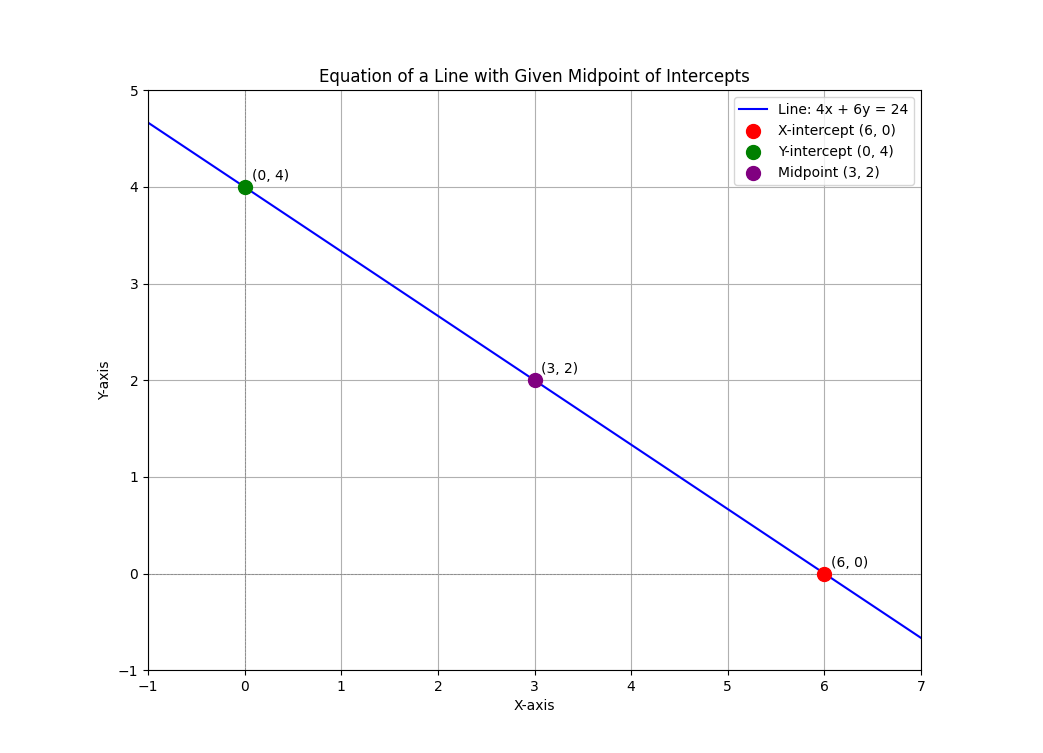
\includegraphics[width=0.7\columnwidth]{figs/fig1.png}
\caption{}
\label{fig:1}
\end{figure}

\end{document}
